\begin{flushleft}
    Wie in unserer Evaluation der Lösungsideen bereits beschrieben übernimmt der ESP32 Microcontroller, siehe Abbildung \ref{fig:esp32_mc}, die Steuerung unseres Roboters. 
    
    \begin{figure}[h!]
        \centering
        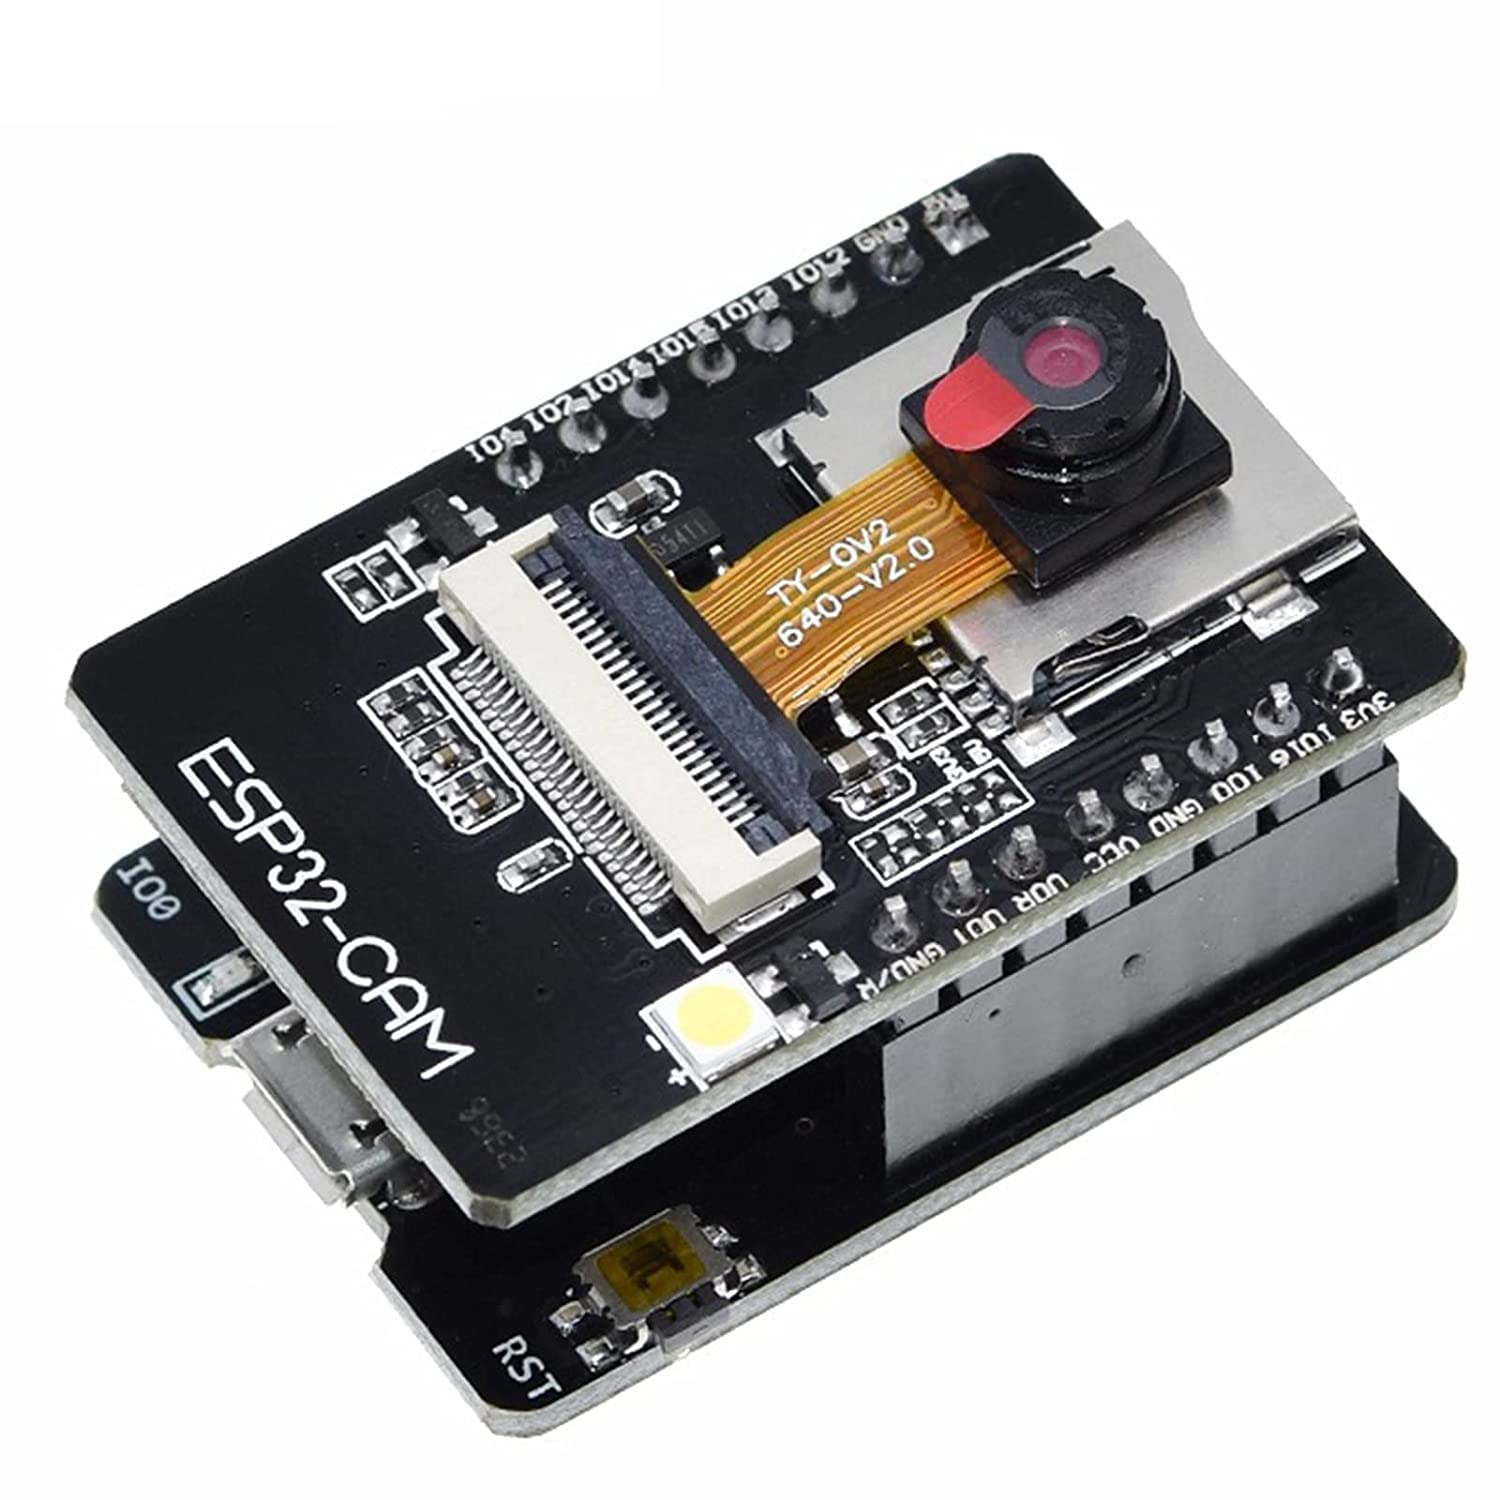
\includegraphics[width=0.3\textwidth]{imgs/Roboter/Real/esp32.jpg}
        \caption{ESP32 Microcontroller}
        \label{fig:esp32_mc}%
    \end{figure}

    Da es sich beim Differentialantreib nur um eine Mechanische Anordnung der Motoren selbst handelt, musste noch ein
    geeignetes Bauteil als Motor selbst gefunden werden.
    Die Motoren müssen ein recht hohes Drehmoment aber eine kleine Umdrehungszahl pro Minute aufweisen.
    Initial war es deshalb die Idee für normale 5V Motoren wie sie auch in DVD Laufwerken verwendet werden ein kleines
    Getriebe zu konzeptionieren und zu bauen.

    \begin{figure}[h!]
        \centering
        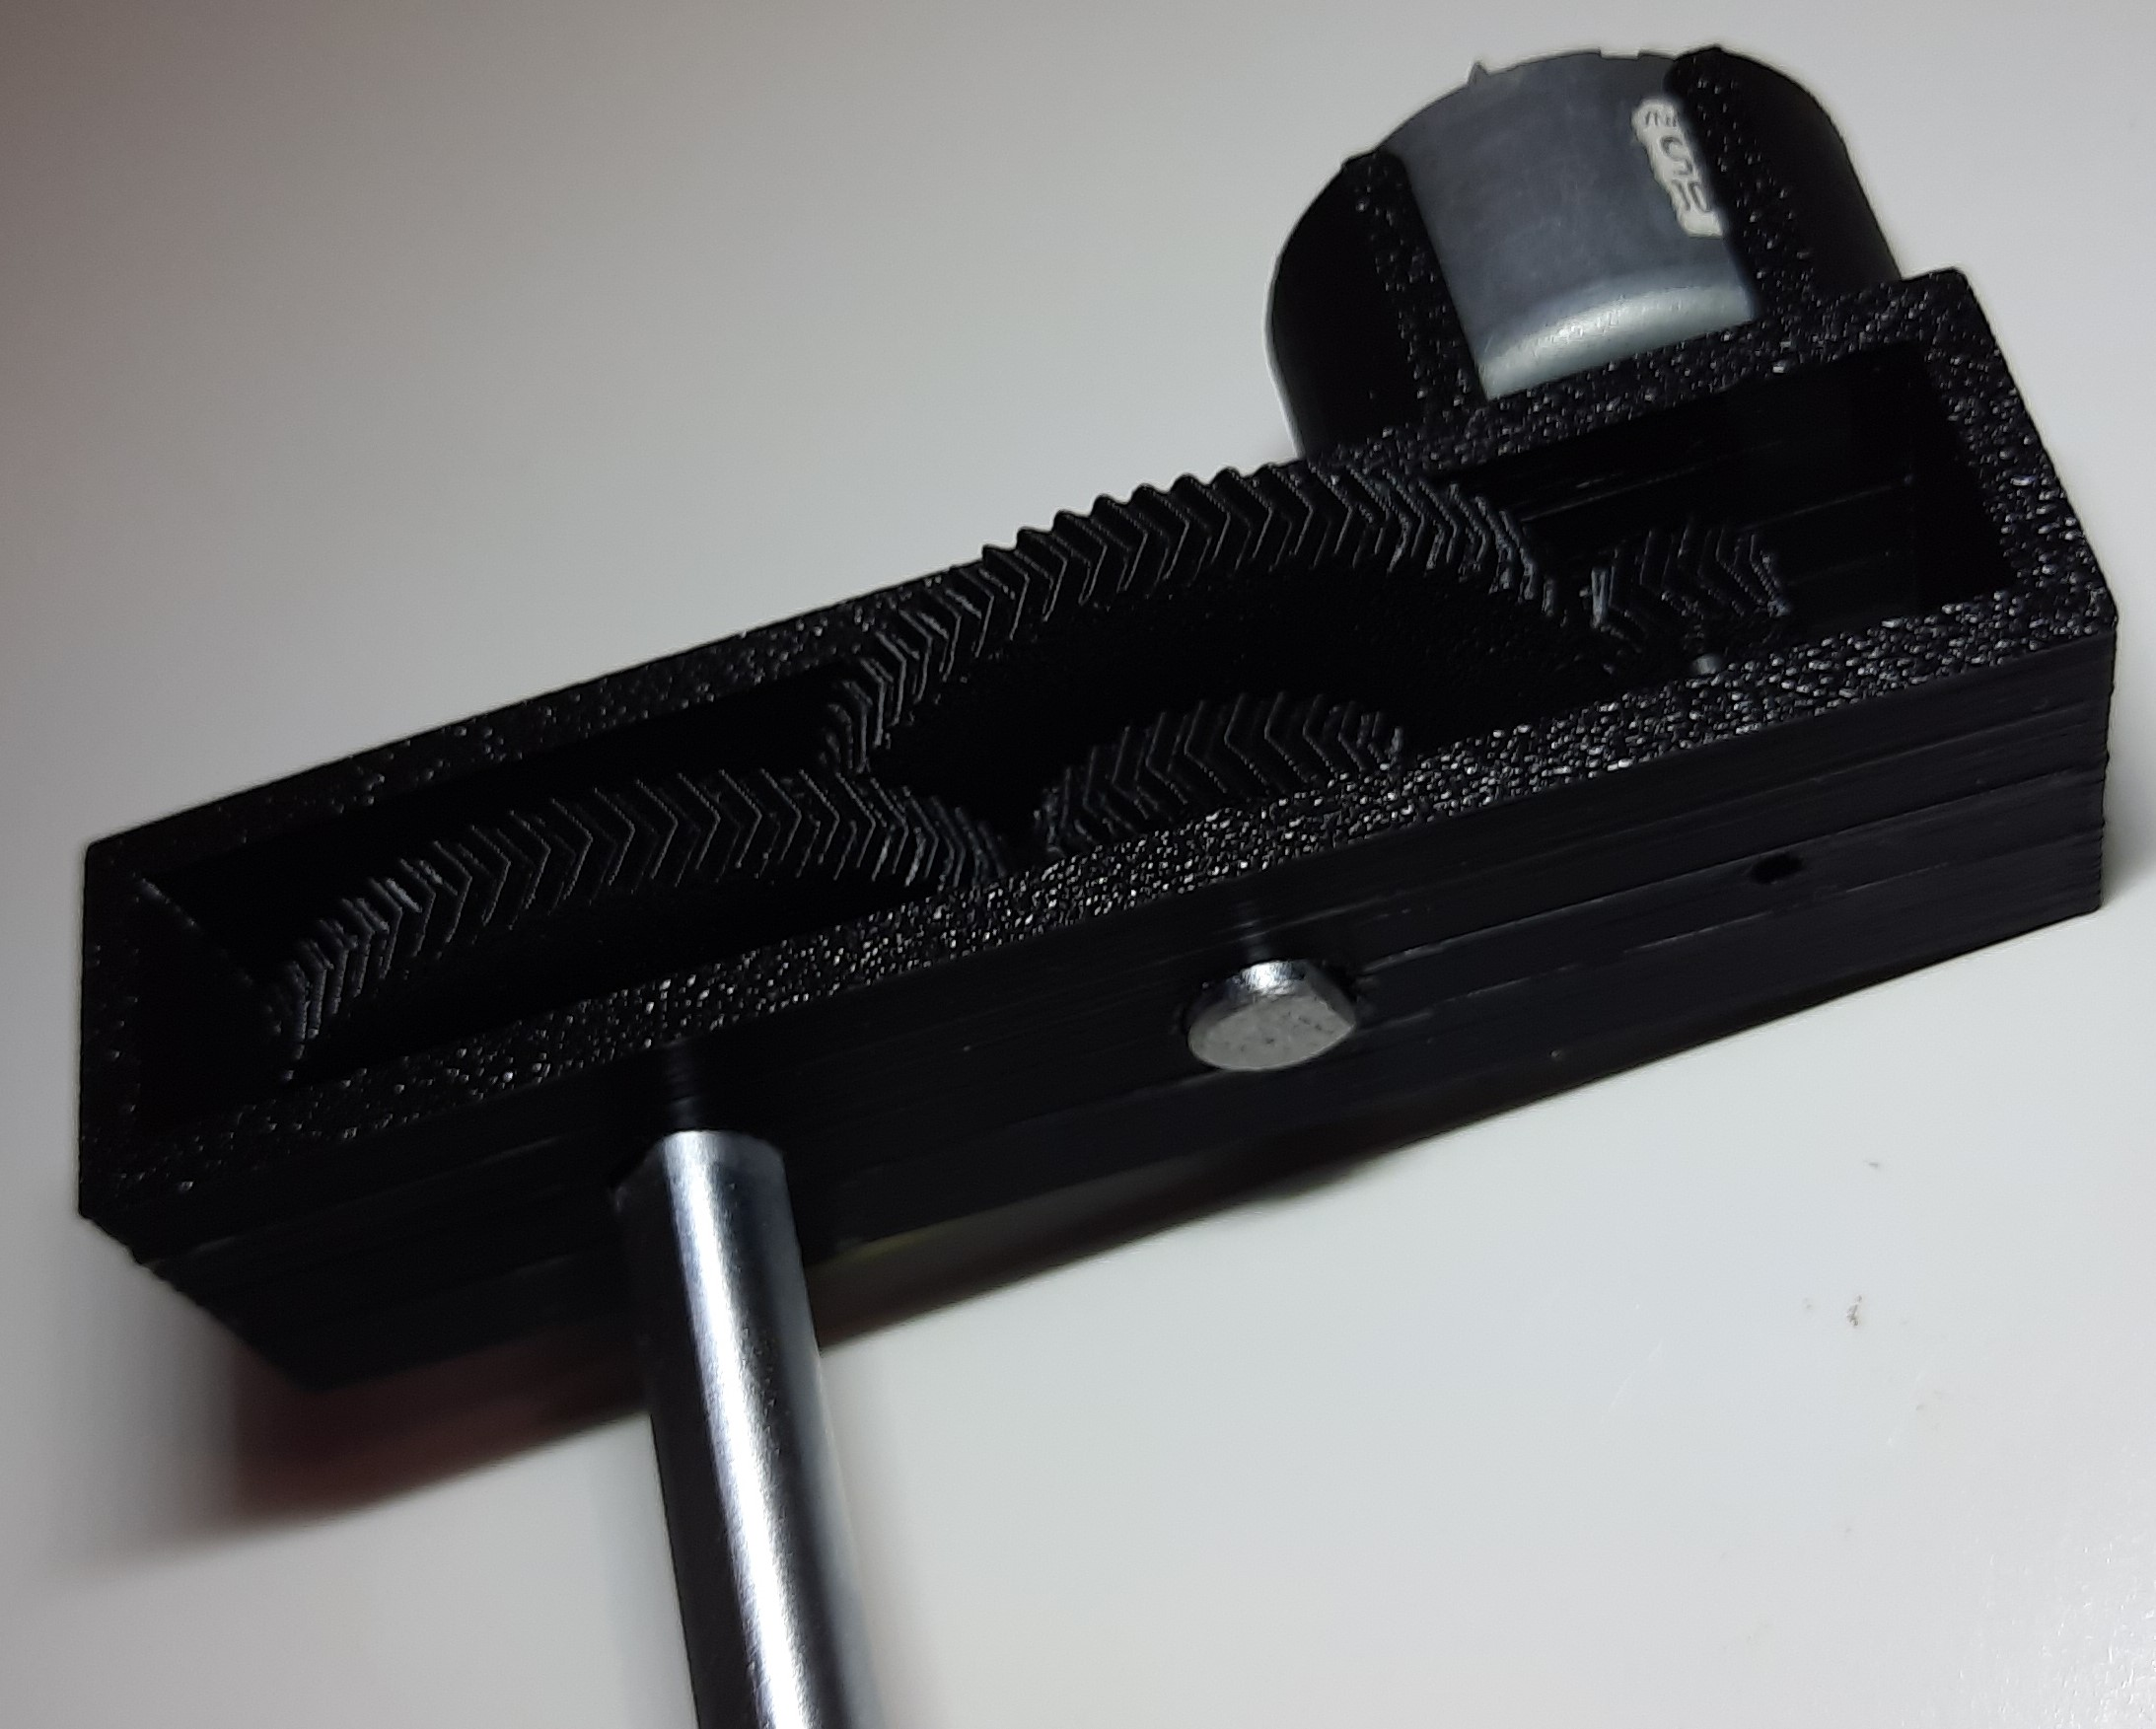
\includegraphics[width=0.3\textwidth]{imgs/Roboter/Real/Getriebe.jpg}
        \caption{Prototyp des eigenbau Motorgetriebe}
        \label{fig:prototyp_transmission}%
    \end{figure}

    Die Idee bewies sich aber recht schnell als zu schwierig und wurde deshalb fallen gelassen.
    Als Ersatz für unseren Misslungenen Versuch fiel die Entscheidung auf Modellbau Getriebemotoren. Siehe Abbildung \ref{fig:robot_motor}.

    \begin{figure}[h!]
        \centering
        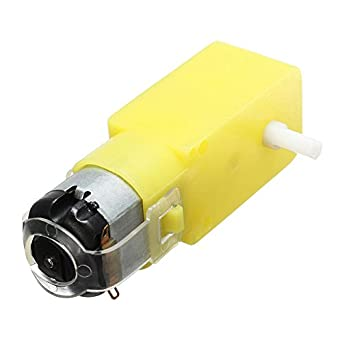
\includegraphics[width=0.3\textwidth]{imgs/Roboter/Real/41eJJZ8mOOL._SX342_.jpg}
        \caption{Modelbau Getriebemotor}
        \label{fig:robot_motor}%
    \end{figure}

    Ein Anforderung an unsere Demo Roboter Platform war die 3D-Druckbarkeit, sowie deren Modularer Aufbau.
    Das Fahrgestell unseres Roboters setzt sich aus insgesamt 3 Modulen zusammen.
    Die Motorenhalterung woran die Motoren selbst und auch die H-Brücke befestigt sind.
    Die Zentrale Platform für unseren Microcontroller.
    Und die beiden Freirollen an der Front des Roboters.

    Dieser muss natürlich auch mit Spannung versogt werden.
    Der Akku unseres Roboter sind sogenannte 18650 LiIon Akkus, diese sind wiederaufladbar und haben die perfekte Größe 
    für unseren kleinen Roboter.

    Die Versorgungsspannung für die Motoren kann direkt von unserem Akkupack abgegriffen werden und zur H-Brücke geführt werden.
    Die H-Brücke benötigt genau so wie der ESP32 eine Versorgungsspannung für die Logik.
    Diese sollte laut Datenblatt bei 5V liegen, erlaubt sind aber auch 3V. Was in unserem Fall ideal ist da unser ESP32
    ebenfalls nur mit 3,3V maxmimal versorgt werden darf.

    Die 3,3V Logikspannung werden auf unserer Platine von einem LM317T, einem Lineareren Spannungswandler zur Verfügung gestellt.

    \begin{figure}[h!]
        \centering
        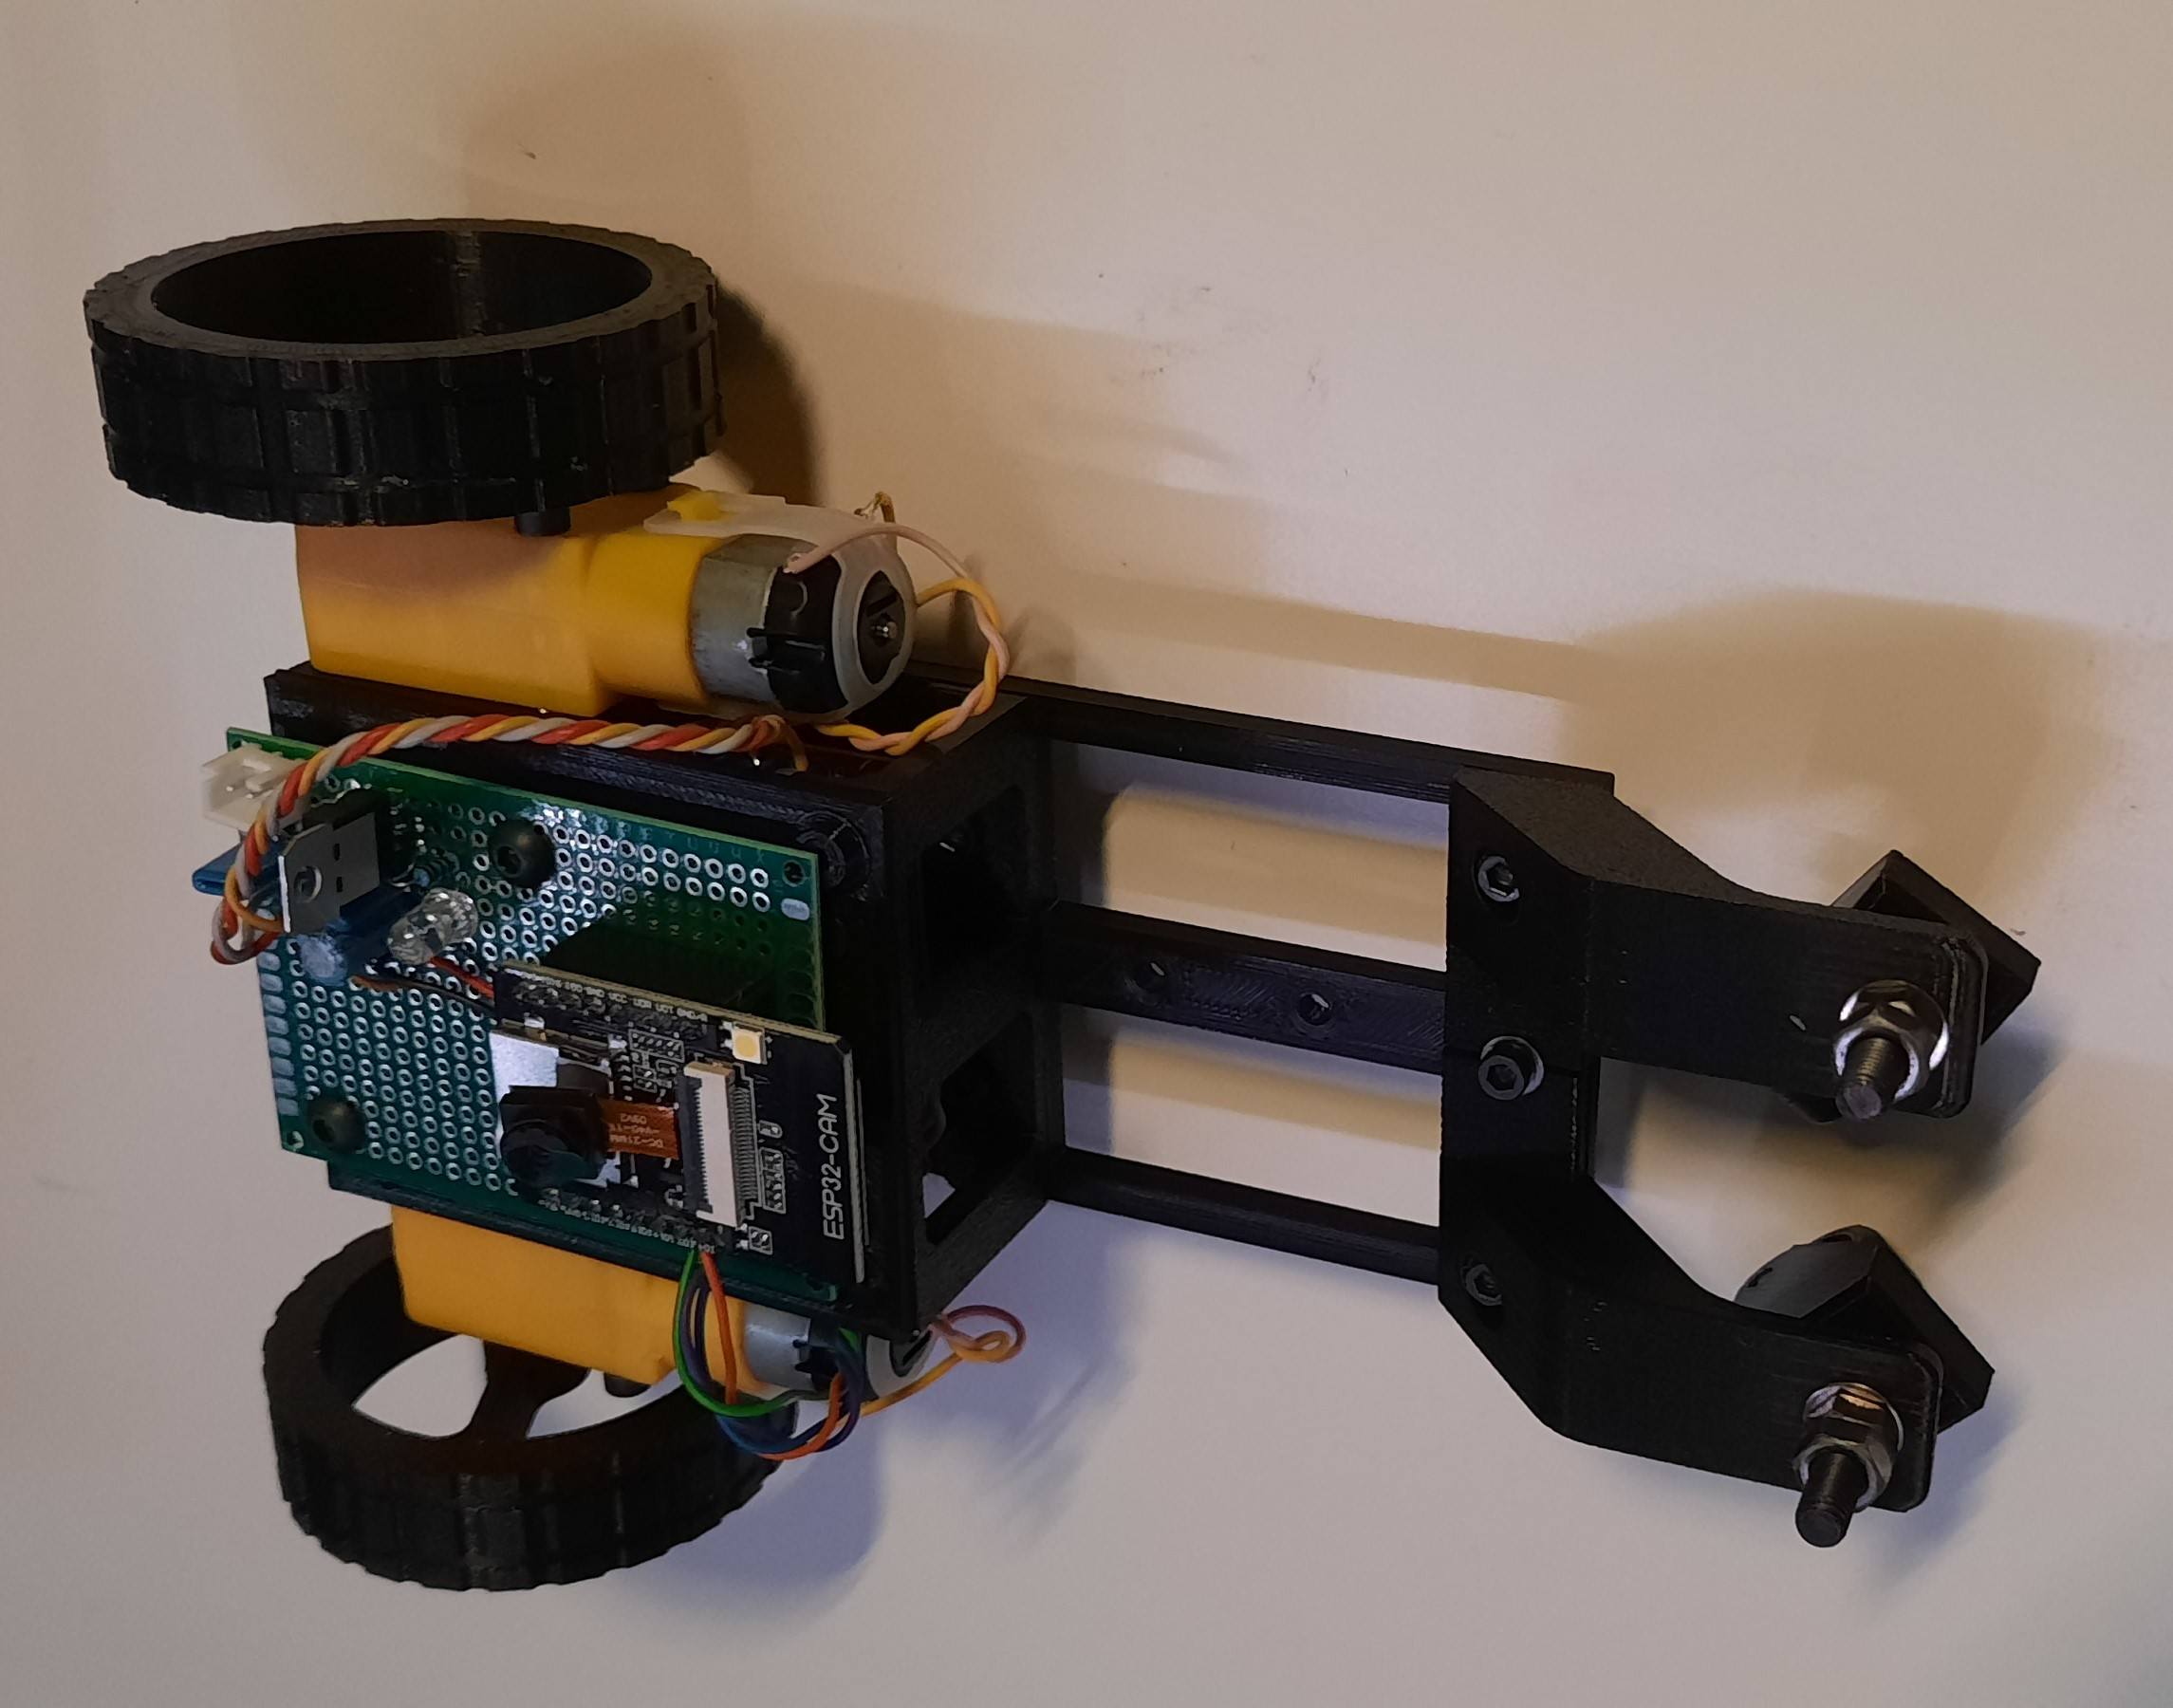
\includegraphics[width=0.5\textwidth]{imgs/Roboter/Real/Roboter.jpg}
        \caption{Roboter Demo Platform}
      \end{figure}

\end{flushleft}